\documentclass[10pt,a4paper]{article}
\usepackage[utf8]{inputenc}
\usepackage[margin=1in]{geometry}
\thispagestyle{empty}

\usepackage{amsmath}
\usepackage{amsfonts}
\usepackage{amssymb}

\usepackage{parskip}

\usepackage{listings}
\usepackage{xcolor}

\usepackage{enumerate}

\usepackage{hyperref}

\usepackage{float}
\usepackage[font=small,labelfont=bf]{caption}
\usepackage{wrapfig}

\usepackage{graphicx}
\restylefloat{figure}

\usepackage{multicol}

\usepackage{cancel}

\author{Cristian Escudero}
\title{Resumen Cálculo Numérico \\ \small{basado en el resumen de Fernando Nellmeldín}}
\begin{document}
\maketitle

\lstset { 
  language=Octave,
  basicstyle=\footnotesize,
  numbers=left,
  numberstyle=\tiny\color{cyan},
  stepnumber=1,
  numbersep=8pt,
  backgroundcolor=\color{white},
  showspaces=false,               % show spaces adding particular underscores
  showstringspaces=false,         % underline spaces within strings
  frame=lines,                   % adds a frame around the code
  rulecolor=\color{cyan},
  tabsize=4,                      
  captionpos=b,                   % sets the caption-position to bottom
  breaklines=true,                % sets automatic line breaking
  keywordstyle=\color{blue},          % keyword style
  commentstyle=\color{gray},       % comment style
  stringstyle=\color{magenta},         % string literal style
}

\section{Métodos Directos}

\subsection{Eliminación de Gauss}
Los elementos de la matriz $A^{(k+1)}$ se calculan:
\begin{align*}
  a_{ij}^{(k+1)} = \left\{ 
  \begin{array}{l l}
    a_{ij}^{(k)} & \quad \text{si $i\leq k$},\\
    a_{ij}^{(k)}-\left(\frac{a_{ik}^{(k)}}{a_{kk}^{(k)}}a_{kj}^{(k)}\right) & \quad \text{si $i \geq k+1$, y $j \geq k+1$},\\
    0 &\quad \text{si $i \geq k+1$, y $j \leq k$}.
  \end{array} \right.
\end{align*}

Si tenemos \textbf{pivoteo parcial}, trabajamos con el \textbf{vector de permutación}:
\begin{lstlisting}
# Se resuelve en n - 1 pasos
for i = 1 : n - 1
	if (parcial)
		# Ponemos la fila con maximo valor
	    [tr, p] = max(abs(Ab(idx(i:n), i)));
	    p = p + i - 1;
    
		if (idx(i) != idx(p))	        
			temp = idx(p);
			idx(p) = idx(i);
			idx(i) = temp;
	    end
	end
	# ... sigue el metodo...
end
\end{lstlisting}

Y trabajamos usando el \texttt{idx(i)} en vez de \texttt{i} para los subíndices.

\small{\underline{Nota}: Si encontramos una columna de ceros, el método no determina una solución \textbf{única}.}

\subsection{Factorización LU}

\begin{align*}
A = \begin{bmatrix}
a_{11} & a_{12} & \cdots & a_{1n} \\
a_{21} & a_{22} & \cdots & a_{2n} \\
\vdots & \vdots & \ddots & \vdots \\
a_{n1} & a_{n2} & \cdots & a_{nn} 
\end{bmatrix} =
\begin{bmatrix}
l_{11} & 0 & \cdots & 0 \\
l_{21} & l_{22} & \ddots & \vdots \\
\vdots & \vdots & \ddots & 0 \\
l_{n1} & l_{n2} & \cdots & l_{nn}
\end{bmatrix}
\cdot
\begin{bmatrix}
u_{11} & u_{12} & \cdots & u_{1n} \\
0 & u_{22} & \cdots & u_{2n} \\
\vdots & \ddots & \ddots & \vdots \\
0 & \cdots & 0 & u_{nn} 
\end{bmatrix} = LU
\end{align*}

Ejemplo 3x3:
\begin{align*}
A=\begin{bmatrix}
a_{11} & a_{12} & a_{13} \\
a_{21} & a_{22} & a_{23} \\
a_{31} & a_{32} & a_{33} 
\end{bmatrix} &=
\begin{bmatrix}
l_{11} & 0 & 0 \\
l_{21} & l_{22} & 0 \\
l_{31} & l_{32} & l_{33} 
\end{bmatrix}
\cdot
\begin{bmatrix}
u_{11} & u_{12} & u_{13} \\
0 & u_{22} & u_{23} \\
0 & 0 & u_{33} 
\end{bmatrix} =LU \\ &=
\begin{bmatrix}
l_{11} \, u_{11} & l_{11} \, u_{12} & l_{11} \, u_{13} \\
l_{21} \, u_{11} & l_{21} \, u_{12} + l_{22} \, u_{22} & l_{21} \, u_{13} + l_{22} \, u_{23}\\
l_{31} \, u_{11} 
& l_{31} \, u_{12} + l_{32} \, u_{22}
& l_{31} \, u_{13} + l_{32} \, u_{23} + l_{33} \, u_{33}
\end{bmatrix}
\end{align*}

\subsubsection{Factorización de Cholesky}
\textit{Nota:} En $a_{ij}^{upper}$: $min(i,j)-1 = i-1$; y en $a_{ij}^{lower}$: $min(i,j)-1 = j-1$.

\begin{align*}
& a_{ij} = \sum_{k=1}^{min(i,j)} l_{ik} \, u_{kj} ,& \\
& a_{ij}^{upper} = \sum_{k=1}^{i-1} l_{ik} \, u_{kj} + l_{ii} \, u_{ij}
&\; \Rightarrow \; u_{ij} = \frac{1}{l_{ii}}\left[ a_{ij} - \sum_{k=1}^{i-1} l_{ik} \, u_{kj} \right]& \\
& a_{ij}^{lower} = \sum_{k=1}^{j-1} l_{ik} \, u_{kj} + u_{jj} \, l_{ij}
&\; \Rightarrow \; l_{ij} = \frac{1}{u_{jj}}\left[ a_{ij} - \sum_{k=1}^{j-1} l_{ik} \, u_{kj} \right]& 
\end{align*}

\begin{align*}
&\text{Factorización de \textbf{Doolittle} ($l_{ii}=1$)}
& u_{ij} = a_{ij} - \sum_{k=1}^{i-1} l_{ik} \, u_{kj}& \\
&\text{Factorización de \textbf{Crout} ($u_{ii}=1$)}
& l_{ij} = a_{ij} - \sum_{k=1}^{j-1} l_{ik} \, u_{kj} & 
\end{align*}

\section{Métodos Iterativos}
Quiero llevar el SEAL a una forma iterativa ($\mathbf{x}=T\mathbf{x}+C$) para poder resolverla:
\begin{align*}
A\mathbf{x} = \mathbf{b} \\
A = D - L - U \\
(D - L - U) \mathbf{x} = \mathbf{b} 
\end{align*}

\begin{align*}
\text{\textbf{\underline{Jacobi}:}} \\
D&\mathbf{x} - (L + U)\mathbf{x} = \mathbf{b} \\
D&\mathbf{x} = (L + U)\mathbf{x} + \mathbf{b} \\
&\mathbf{x} = D^{-1}(L + U)\mathbf{x} + D^{-1}\mathbf{b} \\
&\mathbf{x} = T\mathbf{x} + C \\
\text{\textbf{\underline{Gauss-Seidel}:}} \\
(D-L)&\mathbf{x} - U\mathbf{x} = \mathbf{b} \\
(D-L)&\mathbf{x} = U\mathbf{x} + \mathbf{b} \\
&\mathbf{x} = (D-L)^{-1}U\mathbf{x} + (D-L)^{-1}\mathbf{b} \\
&\mathbf{x} = T\mathbf{x} + C \\
\text{\textbf{\underline{SOR}:}} \\
(D - wL) &\mathbf{x} = [(1-w)D + wU] \mathbf{x} + w \mathbf{b} \\
&\mathbf{x} = (D - wL)^{-1}[(1-w)D + wU] \mathbf{x} + (D - wL)^{-1}w \mathbf{b} \\
&\mathbf{x} = T\mathbf{x} + C 
\end{align*}

\paragraph{Nociones básicas de convergencia:}
\begin{itemize}
\item Si $||T||<1 \;\; \forall ||\cdot|| \Rightarrow$ convergen todos.
\item Si $A$ es e.d.d $\Rightarrow$ converge Jacobi y Gauss-Seidel.
\item Si $A$ es d.p $\wedge\; 0<w<2 \Rightarrow$ SOR converge.
\item $\rho (T) < 1 \iff \mathbf{x}^{(k)}=T\mathbf{x}^{(k-1)} + C$ converge. 
\item ¿$a_{ij} \leq 0 \quad \forall i\neq j \; \wedge \; a_{ii}>0 \quad \forall i$? por \textbf{Teorema 7.22}, tenemos que:
\begin{enumerate}[a.]
\item $0 \leq \rho(T_g) < \rho(T_j)<1$. Si \textit{converge}, G.S. converge más rápido.
\item $1 < \rho(T_j) < \rho (T_g)$. Si \textit{diverge}, G.S. diverge más rápido.
\item $\rho(T_j) = \rho(T_g) = 1$. No convergen.
\end{enumerate}
\end{itemize}

\paragraph{Cotas de error:}
Por \textbf{Corolario 7.20}, tenemos las siguientes \textbf{cotas de error}:
\begin{enumerate}
\item $||\mathbf{x} - \mathbf{x}^{(k)}|| \leq ||T||^{k} ||\mathbf{x}^{(0)}-\mathbf{x}||$;
\item $||\mathbf{x} - \mathbf{x}^{(k)}|| \leq \frac{||T||^{k}}{1-||T||} ||\mathbf{x}^{(1)}-\mathbf{x}^{(0)}||$.
\end{enumerate}

\subsection{Jacobi}

Despejamos $x_i$ del SEAL:
\begin{align*}
a_{11} \, x_1 + a_{12} \, x_2 + a_{13} \, x_3 &= b_1 &\Rightarrow &
&& x_1 = \frac{1}{a_{11}} \left[b_1 - (a_{12} \, x_2 + a_{13}\,x_3)\right]\\
a_{21} \, x_1 + a_{22} \, x_2 + a_{23} \, x_3 &= b_2 &\Rightarrow &
&& x_2 = \frac{1}{a_{22}} \left[b_2 - (a_{21} \, x_1 + a_{23}\,x_3)\right]\\
a_{31} \, x_1 + a_{32} \, x_2 + a_{33} \, x_3 &= b_3 &\Rightarrow &
&& x_3 = \frac{1}{a_{33}} \left[b_3 - (a_{31} \, x_1 + a_{32}\,x_2)\right]\\
\end{align*}
\[x_i^{(k)} = \frac{1}{a_{ii}} \left(b_i - \sum_{\substack{j=1 \\\ i \neq j}}^{n} a_{ij} \, x_j^{(k-1)} \right) \]

\subsection{Gauss-Seidel}
\[x_i^{(k)} = \frac{1}{a_{ii}} \left(b_i - \sum_{j=1}^{i-1} a_{ij} \, x_j^{(k-1)} - \sum_{j=i+1}^{n} a_{ij} \, x_j^{(k-1)} \right) \]

\subsection{SOR (Succesive Over-Relaxation)}
\[x_i^{(k)} = (1-w)\, x_i^{(k-1)} + \frac{w}{a_{ii}} \left(b_i - \sum_{j=1}^{i-1} a_{ij} \, x_j^{(k-1)} - \sum_{j=i+1}^{n} a_{ij} \, x_j^{(k-1)} \right) \]

\subsection{Gradiente Conjugado}
Elige las direcciones de búsqueda ($\mathbf{v}^{(k)}$) durante el proceso iterativo de modo que los $\mathbf{r}^{(k)}$ sean mutuamente ortogonales.
\begin{enumerate}
\item Partimos de un $\mathbf{x}^{(0)}$ y usamos la \textbf{dirección de máximo descenso} $\mathbf{r}^{(0)} = \mathbf{b} - A \mathbf{x}^{0}$ como $\mathbf{v}^{(1)}$.
\item Calculamos el paso de avance $t$ en la dirección $\mathbf{v}$ y la solución aproximada $\mathbf{x}^{(k)}$ (iniciamos con $k = 1$):
\begin{align*}
&t = \frac{<\mathbf{r}^{(k-1)}, \mathbf{r}^{(k-1)}>}{<\mathbf{v}^{(k)},A \mathbf{v}^{(k)}>}, 
&\mathbf{x}^{(k)} = \mathbf{x}^{(k-1)}+t_{k}\mathbf{v}^{(k)}.&
\end{align*}
\item Si $\mathbf{x}^{(k)}$ es la solución de $A\mathbf{x}=\mathbf{b}$ terminamos. Sino calculamos: $\mathbf{r}^{(k)} = \mathbf{b} - t_k A \mathbf{v}^{(k)}$, actualizamos el vector de búsqueda: 
\begin{align*}
&\mathbf{v}^{(k+1)}=\mathbf{r}^{(k)}+s_k\mathbf{v}^{(k)},
&s_k = \frac{<\mathbf{r}^{(k)}, \mathbf{r}^{(k)}>}{<\mathbf{r}^{(k-1)}, \mathbf{r}^{(k-1)}>},&
\end{align*}
y volvemos al paso \textit{2}.
\end{enumerate}

\subsubsection{Precondicionadores}

Para solventar los casos en el que la matriz $A$ a resolver esté mal condicionada, se propone un \textit{precondionamiento}. Es decir, encontrar una matriz $P$ tal que: $\kappa (P^{-1}A)\approx 1$.

\begin{description}
\item \textbf{Jacobi.} El precondicionamiento más simple es: $P = D_s$, con $D_s$ diagonal de $A$. Es efectivo si la matriz es \textbf{diagonal dominante}.
\item \textbf{Block-Jacobi.} Una matriz con bloques de submatrices sobre la diagonal de $A$.
\item \textbf{SOR:} $P= (D_s + w \; L_s) \; D_s^{-1} \; (D_s + w \; U_s)$.
\item \textbf{Cholesky incompleta.} Si A es \textbf{simétrica, definida positiva}, puede descomponerse en: $A = C^T C = {C^*}^T C^* + R$, con $C^*$ una descomposición de \textit{Cholesky} restringida a la estructura rala de A. 
Tomando $P = {C^*}^T C^*$, se espera que el $\kappa$ sea pequeño.
\end{description}

\subsubsection{Criterios de Corte}
Hay varias formas de decidir cuando detener el proceso iterativo:
\begin{itemize}
\item \textbf{Error absoluto:} $||\mathbf{x}^{(k)}-\mathbf{x}^{(k-1)}||\leq \text{tolerancia}_1$. La tolerancia$_1$ depende del significado físico de la variable $\mathbf{x}$.
\item \textbf{Error relativo} $\frac{||\mathbf{x}^{(k)}-\mathbf{x}^{(k-1)}||}{||\mathbf{x}^{(k)}||} \leq \text{tolerancia}_2$. Aquí se es independiente la tolerancia$_2$ de las unidades.
\item \textbf{Error en la aproximación}: $||\mathbf{r}^{(k)}||\leq \text{tolerancia}_3 \cdot ||\mathbf{b}||.$ Es independiente de las unidades debido a que se refiere a la norma del vector de términos independientes.
\end{itemize}

\textbf{@@TODO: Hay un apéndice en la diapositiva de iterativos. Revisar.}

\section{Solución de Ecuaciones No Lineales de una Variable}

\subsection{Método de la Bisección}

El \textit{método de la Bisección} procede buscando una raíz propuesta en la mitad del intervalo $(a,b)$, repitiendo iterativamente el proceso.

\begin{wrapfigure}[10]{r}{0.3\textwidth}
  \label{fig:bisection}
  \caption{\textit{Método de la Bisección}, representación gráfica.}
  \centering
  \hbox{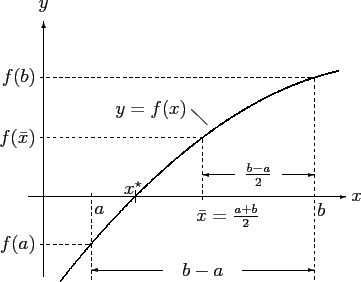
\includegraphics[width=0.3\textwidth-\fboxrule-\fboxrule]{img/bisection.png}}  
\end{wrapfigure}	

Es un método lento, de convergencia \textit{lineal}, pero \textbf{siempre} \textit{converge}. Es \textit{robusto} (siempre encuentra solución), por lo que por esa razón es usado para iniciar otros métodos más eficientes.

Sea $f(x)$ \textbf{contínua} en $[a,b]$ y $f(a)\cdot f(b)<0$. Entonces, por el \textbf{teorema del valor medio}, $\exists \; a<p<b \; / \; f(p) = 0$.

\subsubsection{Algoritmo}
Supongamos $a_1=a$, $b_1=b$, $i=1$.
\begin{enumerate}
\item Calculamos el punto medio $p_i = a_i + \frac{b_i - a_i}{2}=\frac{a_i+b_i}{2}$.
\item Si $f(p_i)=0 \Rightarrow p_i$, encontramos la raíz, y terminamos.
\item Si $f(p_i)\cdot f(a_i)<0$:
\subitem - Entonces, $b_{i+1} = p_i$, y $a_{i+1}=b_i$.
\subitem - De lo contrario, $a_{i+1} = p_i$, y $b_{i+1}=b_i$.
\item Incrementamos $i$, y volvemos al paso \textit{1}.
\end{enumerate}

\setlength{\columnsep}{2cm}
\begin{multicols}{2}
\subsubsection{Criterios de corte}
Siendo una tolerancia $\mathcal{E}>0$:
\begin{itemize}
\item \textbf{Error absoluto:} $|p_i - p_{i-1}| \leq \mathcal{E}$.
\item \textbf{Error relativo:} $\frac{|p_i - p_{i-1}|}{|p_i|} \leq \mathcal{E}$. 

Es independiente de las unidades y del significado físico de estas.
\item \textbf{Error en la aproximación:} $|f(p)| \leq \mathcal{E}$.
\end{itemize}
\vfill
\subsubsection{Cota de error}
Del \textbf{Teorema 2.1}, supongamos que $f \in C[a,b] \wedge f(a)\cdot f(b)<0$, entonces el método genera una sucesión $\{p_n\}_{n=1}^\infty$ que aproxima a un cero de $p$ de $f$, tal que:
\[|p_n - p| \leq \frac{b-a}{2^n}, \text{ con } n \geq 1.\]
Otra cota de error fácilmente calculable (p72), es:
\[|p_n-p| < \frac{1}{2}|a_n - b_n|.\]
\end{multicols}

\pagebreak

\subsection{Iteración de Punto Fijo}

\begin{figure}[h!]
  \caption{\textit{Iteración de Punto Fijo}, \textbf{convergencia} por $|g'(x)|<1$ (izquierda), \textbf{divergencia} por $g'(x)<-1$ (medio), y por $|g'(x)|>1$(derecha).}
  \label{fig:puntofijo}
  \centering
  \hbox{
  	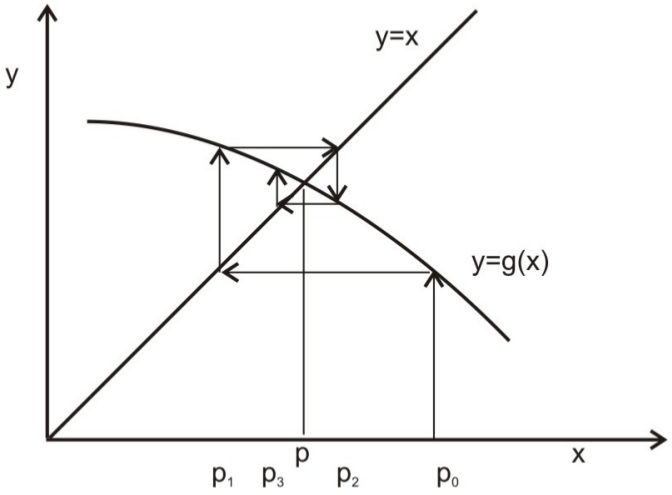
\includegraphics[width=0.3\textwidth-\fboxrule-\fboxrule]{img/puntofijo1.png}
	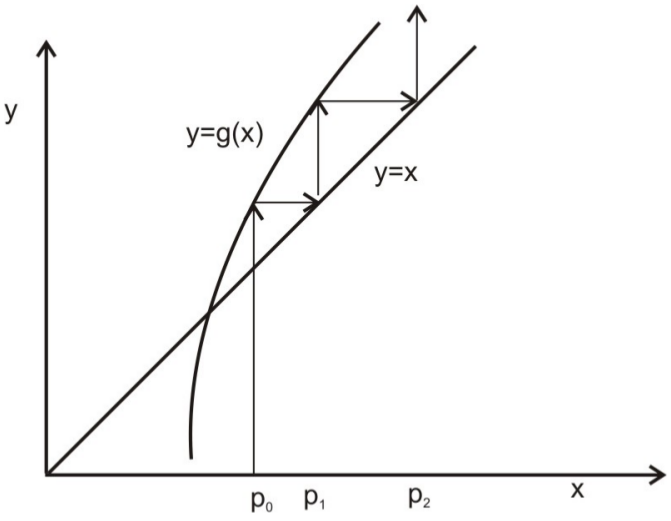
\includegraphics[width=0.3\textwidth-\fboxrule-\fboxrule]{img/puntofijo2.png}  
	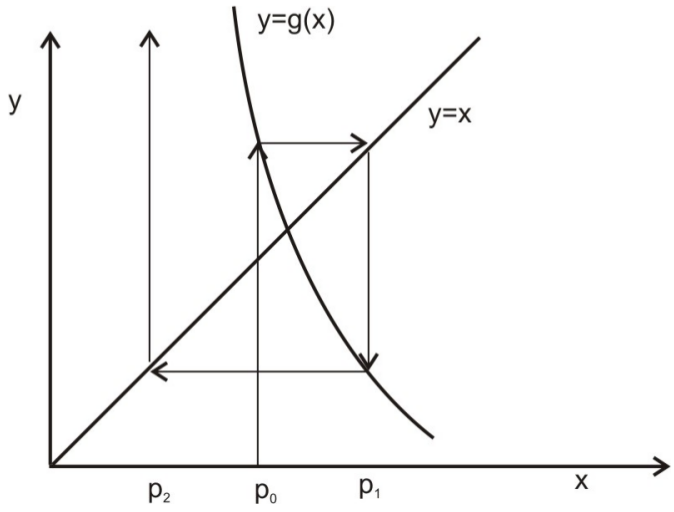
\includegraphics[width=0.3\textwidth-\fboxrule-\fboxrule]{img/puntofijo3.png} }
\end{figure}

\setlength{\columnsep}{2cm}
\begin{multicols}{2}
\subsubsection{Algoritmo}
\begin{enumerate}
\item Se escoge una aproximación inicial $p_0$.
\item Se genera la sucesión $\{p_n\}_{n=1}^\infty$, \\con $p_n = g(p_{n-1})$.
\item Si la sucesión converge en $p$ y si $g$ es continua, entonces:
\[p=\lim_{n\rightarrow \infty} p_n = \lim_{n\rightarrow \infty} g(p_{n-1})=g(\lim_{n\rightarrow \infty} p_{n-1})=g(p),\]
y obtenemos una solución con $p=g(p)$.
\end{enumerate}
\vfill 

\subsubsection{Cotas de error}
Están dadas por el \textbf{Corolario 2.4}. Las cotas de error que supone utilizar $p_n$ para aproximar $p$ están dadas por:
\[|p_n - p| \leq k^n \max \{p_0 -a, b - p_0\},\]
y por:
\[|p_n - p| \leq \frac{k^n}{1-k} |p_1 - p_0|, \quad \forall n\geq 1.\]
\end{multicols}
\setlength{\columnsep}{10pt}

\subsection{Método de Newton-Raphson}

Sea $f \in C^2 [a,b]$, el método construye una sucesión $\{p_n\}$ con la siguiente fórmula de recurrencia:
\[p_n = p_{n-1} - \frac{f(p_{n-1})}{f(p_{n-1})},\quad n\geq 1.\]

\textbf{Convergencia:} está dada por el \textbf{teorema $2.5$}.

\subsubsection{Cota de error (diapositiva):}
\[e_{n+1}=|p_{n+1}-p| \approx e_n^2\frac{f''(p)}{2f'(p)} = C e_n^2.\]

\textit{Nota:} Ver además \textbf{Teorema 2.8}. De el concluímos que otra cota de error es (cumplidas las hipótesis):
\[|p_{n+1}-p| < \frac{M}{2}|p_n - p|^2.\]

\subsubsection{M.N.R. con raíces múltiples (p84):}
\[g(x)=x-\frac{f(x) f'(x)}{[f'(x)]^2 -f(x) f''(x)}.\]

\begin{figure}[h!]
  \label{fig:newton}
  \caption{Método de Newton-Raphson (\textit{izquierda}), método de la Secante (\textit{derecha}).}
  \centering
  \hbox{
  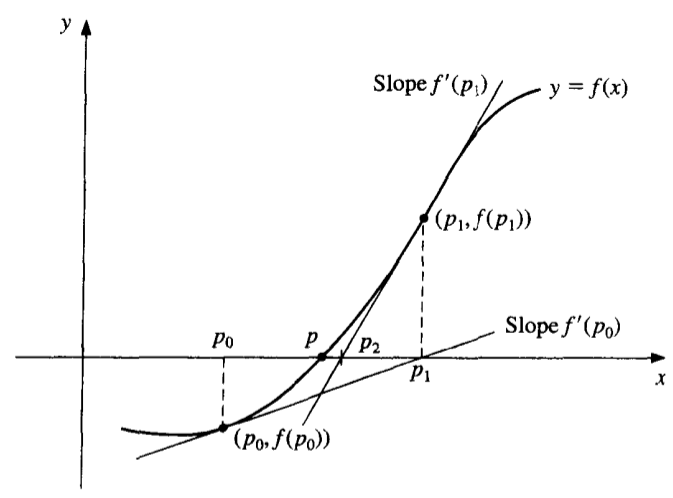
\includegraphics[width=0.45\textwidth-\fboxrule-\fboxrule]{img/newton.png}
  \hspace{0.04\textwidth-\fboxrule-\fboxrule}
   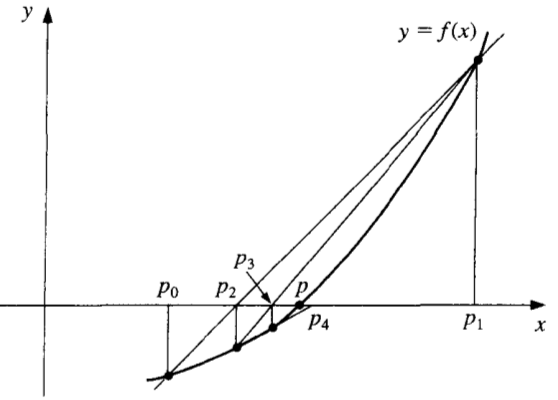
\includegraphics[width=0.45\textwidth-\fboxrule-\fboxrule]{img/secant.png}
    }
\end{figure}	

\subsection{Método de la Secante}

Para solventar el problema del \textit{método de Newton} de desconocer la derivada de la función, se utiliza este método.

La fórmula de recurrencia, basada en la definición de derivada, está dada por:
\[p_{n+1} = p_{n} - \frac{p_{n}-p_{n-1}}{f(p_{n})-f(p_{n-1})}f(p_{n}) .\]

La \textbf{convergencia} es \textit{superlineal}: $e_{n+1}=C \; e_n^{1.618...}$.

Requiere además dos estimaciones iniciales $p_0$ y $p_1$.

\subsection{Método de la Falsa Posición}

Similar al \textit{método de la secante}, pero en cada iteración toma -para trazar la secante- los dos últimos puntos que acotan la raíz buscada (como el \textit{método bisección}).

Para determinar el punto que uso, evalúo: 
\[f(p_n)\cdot f(p_{n-1}) < 0,\]
Si es \textbf{verdadero}, uso $p_{n-2}$, sino $p_{n-1}$, para seleccionar el intervalo con ${p_n}$.

\pagebreak
\section*{CheatSheet}

\begin{multicols}{2}
\begin{enumerate}
\item \textbf{Operaciones en Matriz:}
\begin{itemize}
\item $(E_i) \leftrightarrow E_j$.
\item $(\lambda E_i)  \rightarrow E_i$.
\item $(E_i + \lambda E_j) \rightarrow E_i$.
\end{itemize}
%
\item \textbf{Afirmaciones equivalentes (6.16):}
\begin{itemize}
\item $A\mathbf{x}=\mathbf{0} \iff \mathbf{x}=\mathbf{0}$.
\item $A\mathbf{x}=\mathbf{b} \text{ tiene solución única}$.
\item $\exists A^{-1} (A \text{ es no \textit{singular}})$.
\item $\det A \neq 0$.
\item Se puede \textit{gaussear}.
\end{itemize}
%
\item \textbf{Factorización LU}: \\
$\exists$ si \textit{gausseamos} sin intercambio de renglones.
%
\item \textbf{Resolver LU:} 
\[A\mathbf{x}=\mathbf{b} \rightarrow A=LU \rightarrow LU\mathbf{x}=\mathbf{b} \]
\[ \rightarrow U\mathbf{x}=\mathbf{y}\rightarrow L\mathbf{y}=\mathbf{b}\]
%
\item \textbf{Eliminación de Gauss:}
\begin{align*}
  a_{ij}^{(k+1)} = \left\{ 
  \begin{array}{l l}
    a_{ij}^{(k)} & \text{si $i\leq k$},\\
    0 & \text{si $i \geq k+1$, $j \leq k$},\\
  \end{array} 
  \right.
\end{align*}
En otro caso, $a_{ij}^{(k)}-\left(\frac{a_{ik}^{(k)}}{a_{kk}^{(k)}}a_{kj}^{(k)}\right)$.
\item \textbf{Estrategias de pivoteo:}
\begin{itemize}
\item \textbf{Simple}: buscar $a^{(k)}_{pk}\neq 0$.
\item \textbf{Parcial}: buscar $a^{(k)}_{pk}$ con máximo \texttt{abs}.
\item \textbf{Parcial Escalado}: buscar el pivote más grande en relación con su fila.
\end{itemize}
%
\item \textbf{Estrictamente Diagonal Dominante:}
\[|a_{ii}|>\sum_{j=1, \, i\neq j}^n |a_{ij}|, \quad \forall i \in [1,n].\]
%
\item \textbf{Definida Positiva:} Si es simétrica, y:
\[\mathbf{x}^T A \mathbf{x} > 0 \quad \forall \mathbf{x} \neq \mathbf{0}.\]
%
\item \textbf{Sea $A$ e.d.d:}
\begin{itemize}
\item Es \textbf{no singular}.
\item Tiene solución \textbf{única}.
\item No se necesitan intercambio de renglones (tiene factorización $LU$).
\end{itemize}
%
\columnbreak
\vfill
\item \textbf{Sea $A$ definida positiva:}
\begin{itemize}
\item A es \textbf{no singular.}
\item $a_{ii} >0 \quad \forall i$.
\item $(a_{ij})^2 < a_{ii} a_{jj} \quad \forall i \neq j$.
\item $\smash{\displaystyle\max_{1\leq i,j \leq n}} |a_{ij}| \leq \smash{\displaystyle\max_{1\leq i \leq n}} |a_{ii}|$.
\\
\item $\lambda_{i}>0 \quad \forall i$.
\item Podemos \textit{gaussear} sin intercambio de renglones (tiene factorización $LU$) y los pivotes son positivos.
\item Y, ¿es simétrica? $\iff \det(A_k) >0 \; \forall k$.
\item Y, ¿$A$ es matriz $\mathbb{R}$? $\Rightarrow$ tiene factorización \textbf{única} $A = CC^T$, y $A=LDL^T$ con $L_{ii} =1$ y $D_{ii}>0$.
\end{itemize}
%
\item \textbf{Norma vectorial:}
\begin{itemize}
\item $||\mathbf{x}||>0$.
\item $||\mathbf{x}||=0 \iff \mathbf{x}=\mathbf{0}$.
\item $||\alpha \mathbf{x}|| = |\alpha | \cdot ||\mathbf{x}||$.
\item $||\mathbf{x}+\mathbf{y}|| \leq ||\mathbf{x}||+||\mathbf{y}||$. 
\\
\item \textbf{Euclídea}: $||\mathbf{x}||_2 = \left(\sum x_i^2\right)^{1/2}$.
\item \textbf{Infinito}: $||\mathbf{x}||_\infty = \max \{|x_i|\}$.
\item \textbf{L1}: $||\mathbf{x}||_1 = \sum |x_i|$.
\end{itemize}
%
\item \textbf{Norma matricial:}
\begin{itemize}
\item Ídem \textit{norma vectorial} pero con matrices.
\item $||A||=\max ||A \mathbf{x}||$ con $||\mathbf{x}||=1$.
\item $||A \mathbf{z}|| \leq ||A||\cdot||\mathbf{z}||$.
\item $||AB||\leq ||A||\cdot ||B||$.
\item ¿$A$ es matriz \textbf{cuadrada}? \\$\Rightarrow ||A||_\infty = \max \left\lbrace\sum |a_{ij}|\right\rbrace$.
\end{itemize}
%
\item \textbf{Eigenvalue ($\lambda$):} $(A-\lambda I) = 0$.
%
\item \textbf{Radio espectral:} $\rho(A) = \max|\lambda_i|$.
%
\item \textbf{Número de Condición:}
\begin{itemize}
\item $\kappa (A)= ||A|| \cdot ||A^{-1}|| = \frac{\lambda_{\max}}{\lambda_{\min}}$.
\item Si $\kappa \approx 1 \Rightarrow$ \textbf{bien} condicionada.
\item Si $\kappa >> 1 \Rightarrow$ \textbf{mal} condicionada.
\end{itemize}
%
\item \textbf{Afirmaciones equivalentes (7.17):}
\begin{itemize}
\item $A$ es una matriz \textbf{convergente}.
\item $\lim_{n\rightarrow \infty} ||A^{(n)}||=0 \quad \forall ||\cdot||$.
\item $\lim_{n\rightarrow \infty} A^{(n)} \mathbf{x}=\mathbf{0} \quad \forall \mathbf{x}$.
\item $\rho(A) < 1$.
\end{itemize}
%
\end{enumerate}

\end{multicols}

\end{document}